%Author: Giacomo Fabris

\documentclass[11pt,a4paper,openany]{memoir}
\usepackage{mdframed}
\usepackage{ntheorem}
\usepackage{lipsum}
\usepackage[inline]{enumitem}
\usepackage{amssymb}
\usepackage{indentfirst}
\usepackage{calrsfs}
\usepackage[]{algorithm2e}
\usepackage{mathtools}
\usepackage[mathcal,mathscr]{eucal}
\usepackage{float}
\usepackage{cancel}

\usepackage{tikz}
\usetikzlibrary{graphs, graphs.standard, quotes}% quotes library is for the [""] edges

\theoremstyle{break}\usepackage[italian,english]{babel}
\usepackage[utf8]{inputenc}

\theoremstyle{break}
\newtheorem{definition}{Definizione}
\newenvironment{fdefinition}
  {\begin{mdframed}\begin{definition}}
  {\end{definition}\end{mdframed}}
\chapterstyle{dash}

\setlist[itemize]{noitemsep, topsep=0pt}
\setlist[enumerate]{noitemsep}



\begin{document}

\begin{titlingpage} % Suppresses displaying the page number on the title page and the subsequent page counts as page 1
	
	\raggedleft % Right align the title page
	
	\rule{1pt}{\textheight} % Vertical line
	\hspace{0.05\textwidth} % Whitespace between the vertical line and title page text
	\parbox[b]{0.75\textwidth}{ 
		{\Huge\bfseries Appunti di Logica}\\[4\baselineskip]
		{\large\textit{Sul corso di Logica Matematica @ DISI,\\ Università degli Studi di Trento}}\\\\
		{\textsc{A.A. 2018/2019}\\[3\baselineskip]
		%\texttt{github.com/gik98/unitn18-logics}
		}
		
		\vspace{0.4\textheight}
		
		\texttt{github.com/gik98/unitn18-logics}
		
	}

\end{titlingpage}

\chapter{PL - Introduzione}
La logica delle proposizioni (Propositional Logic -\textbf{PL}) è una logica che permette di rappresentare fatti (affermazioni), che possono essere vere o false.

PL si compone di \textbf{simboli logici} e \textbf{variabili proposizionali}. Una proposizione (formula) è composta quindi di variabili proposizionali uniti da simboli logici. La formula può essere \textit{vera} o \textit{falsa} a seconda dell'assegnazione delle singole variabili.

\begin{fdefinition}[Linguaggio della PL]
\textbf{Logical symbols:}
\begin{enumerate*}[label=(\arabic*)]
\item $\lnot$
\item $\land$
\item $\lor$
\item $\supset$
\item $\equiv$
\end{enumerate*}
\\
\textbf{PL formulas and sub-formulas}
\begin{itemize}
\item every logical variable $P \in \mathrm{P}$ is an atomic formula
\item every atomic formula is a formula
\item if A and B are formulas, then $\lnot A, A \land B, A \lor B, A \supset B, A \equiv B$ are formulas
\end{itemize}
\end{fdefinition}

Una \textbf{funzione di interpretazione} $I: \mathit{P} \to \lbrace \top, \bot \rbrace$ assegna un valore vero o falso a ciascuna variabile $P \in \mathrm{P}$.

Una funzione di interpretazione è detta \textbf{modello} di una funzione $\varphi$ se le sue assegnazioni rendono il valore della funzione vero. In simboli: $I \models \varphi$.

\subsection{SAT, UNSAT, VAL}

\begin{itemize}
\item Una formula $\mathrm{A}$ è soddisfacibile (\textbf{SAT}) se $\exists I$ funzione di interpretazione t.c. $I \models \mathrm{A}$.

\item Una formula $\mathrm{A}$ è insoddisfacibile (\textbf{UNSAT}) se $\nexists I$ funzione di interpretazione t.c. $I \models \mathrm{A}$.

\item Una formula $\mathrm{A}$ è valida (\textbf{VALID}) se $\forall I, I \models \mathrm{A}$
\end{itemize}

\textbf{Osservazione:}

Se $\mathrm{A}$ è \textbf{VALID}, $\lnot \mathrm{A}$ è \textbf{UNSAT}.

Se $\mathrm{A}$ è \textbf{SAT}, $\lnot \mathrm{A}$ non è valida.

Se $\mathrm{A}$ non è valida, $\lnot \mathrm{A}$ è \textbf{SAT}.

Se $\mathrm{A}$ è \textbf{UNSAT}, $\lnot \mathrm{A}$ è \textbf{VALID}. 


\subsection{Conseguenza e equivalenza logica}
\begin{itemize}
\item Una formula $\mathrm{A}$ è una \textbf{conseguenza logica} di un insieme di formule $\Gamma$, in simboli $\Gamma \models \mathrm{A}$ sse per ogni funzione di interpretazione $I$ che soddisfa tutte le formule di $\Gamma$, $I$ soddisfa $\mathrm{A}$.

\item Due formule $\mathrm{A}, \mathrm{B}$ sono \textbf{equivalenti}, in simboli $\mathrm{A} \equiv \mathrm{B}$ sse per ogni funzione di interpretazione $I$, $I(\mathrm{A}) = I(\mathrm{B})$. 
\end{itemize}

\subsection{Procedure di decisione}

\textbf{Model checking ($I$, $\varphi$)}: $I \stackrel{?}{\models} \varphi$ ($I$ soddisfa $\varphi$?)

\textbf{Satisfiability ($\varphi$)}: $\stackrel{?}{\exists} I | I \models \varphi$ (Esiste un modello che soddisfi $\varphi$?)

\textbf{Validity ($\varphi$)}: $\stackrel{?}{\models} \varphi$ ($\varphi$ è soddisfatta da qualsiasi modello?)

\textbf{Logical consequence ($\Gamma$, $\varphi$)}: $\Gamma \stackrel{?}{\models} \varphi$ (Ogni modello che soddisfa $\Gamma$ soddisfa anche $\varphi$?)

\subsection{Formalizzazione del linguaggio naturale}

\begin{itemize}
\item $A$: "It is the case that A"
\item $\lnot A$: "It is not the case that A"
\item $A \land B$: "A and B", "A but B", "Although A, B", "Both A and B"
\item $A \lor B$: "A or B", "Either A or B"
\item $A \to B$: "If A, then B", "B if A"
\item $\lnot (A \lor B)$: "Neither A nor B"
\item $\lnot (A \land B)$: "It is not the case that both A and B"
\end{itemize}
\chapter{PL - CNF \& DPLL}

\chapter{PL - Tableaux}

\subsection{Regole di riduzione}

\begin{tabular*}{\textwidth}{c @{\extracolsep{\fill}} c}
$\alpha$ rules & $\lnot \lnot$ elimination \\
\\
%alpha rules
\begin{tabular}{c c c}
\begin{tabular}{c}
$\phi \land \psi$ \\
\hline
$\phi$ \\
$\psi$ \\
\end{tabular} &
\begin{tabular}{c}
$\lnot (\phi \lor \psi)$ \\
\hline
$\lnot \phi$ \\
$\lnot \psi$ \\
\end{tabular} &
\begin{tabular}{c}
$\lnot (\phi \supset \psi)$ \\
\hline
$\phi$ \\
$\lnot \psi$ \\
\end{tabular}
\end{tabular} &
%lnot lnot elimination
\begin{tabular}{c}
$\lnot \lnot \phi$ \\
\hline
$\phi$
\end{tabular}\\
\\
$\beta$ rules & Branch closure \\
%beta rules
\begin{tabular}{c c c}
\begin{tabular}{c}
$\phi \lor \psi$ \\
\hline
$\phi$ \vline \hspace{1mm} $\psi$ 
\end{tabular} &
\begin{tabular}{c}
$\lnot (\phi \land \psi)$ \\
\hline
$\lnot \phi$ \vline \hspace{1mm} $\lnot \psi$ 
\end{tabular} &
\begin{tabular}{c}
$\phi \supset \psi$ \\
\hline
$\lnot \phi$ \vline \hspace{1mm} $\psi$ 
\end{tabular}
\end{tabular} &
%branch closure
\begin{tabular}{c}
$\phi$\\
$\lnot\phi$\\
\hline
$\mathrm{X}$
\end{tabular}\\
\end{tabular*}

L'equivalenza può essere riscritta come doppia implicazione.

$$\phi \equiv \psi \iff (\phi \supset \psi) \land (\psi \supset \phi)$$

\noindent\hrulefill
\vspace{1em}

\textbf{Osservazione:} le $\alpha$- e $\beta$ rules del tableaux sono analoghe a quelle di riduzione in \textit{CNF}:
\begin{itemize}
\item una $\alpha$ rule è equivalente a and logico $\land$ delle formule da ridurre;
\item una $\beta$ rule è equivalente a or logico (nella forma $\otimes$) fra tutte le formule da ridurre, prese a due a due.
\end{itemize}

\subsection{Metodo del tableaux}
Il \textbf{tableaux} è un metodo per provare se un insieme di formule dato è \textbf{insoddisfacibile}. Di conseguenza, è possibile dimostrare anche la \textbf{validità} dell'insieme di formule (dimostrando l'insoddisfacibilità della negazione dell'insieme di formule).

Il \textbf{tableaux} costruisce un albero binario, la cui radice è la congiunzione dell'insieme di formule di cui si vuole verificare l'insoddisfacibilità. Nuove foglie sono aggiunte applicando $\alpha$ rules (\textit{deterministic rules}) o $\beta$ rules (\textit{branch splitting})a una qualsiasi formula che appare in un nodo \textit{ancestor}. 

Un ramo dell'albero è \textbf{chiuso} se il cammino fra la foglia e la radice contiene formule contraddittorie (es. $p$, $\lnot p$). Se tutti i rami possono essere chiusi, allora la formula di partenza è insoddisfacibile.

\textbf{Osservazione:} è conveniente applicare $\alpha$ rules anziché $\beta$ rules, laddove possibile, in modo da non aumentare il numero di rami dell'albero.

\subsection{Interpretazione dal tableaux}
Si può dimostrare che un tableaux in PL termina sempre (dopo un numero finito di passi tutti i rami sono chiusi oppure tutte le formule che compaiono nel tableaux sono state valutate). Pertanto, se una formula genera un tableaux che non si chiude, la formula è \textbf{soddisfacibile}.

I modelli che rendono il tableaux soddisfacibile possono essere ricavati dai rami rimasti aperti. Per ogni ramo e per ogni variabile proposizionale $p$, vale $I(p) = \top$ se nel cammino dalla foglia alla radice compare $p$; $I(p) = \bot$ se nel cammino dalla foglia alla radice compare $\lnot p$. Se né $p$ né $\lnot p$ compaiono, $I(p)$ può essere definito arbitrariamente (entrambe le definizioni renderanno la formula soddisfacibile).
\chapter{FOL - Introduzione}

La logica del primo ordine (First-Order Logic - \textbf{FOL}) è un'estensione della propositional logic.

Mentre la PL prevede solamente valori di verità o falsità, FOL prevede \textit{variabili} che rappresentano oggetti del mondo da descrivere, inoltre, questi oggetti possono essere quantificati (si possono descrivere \textit{tutti} gli oggetti o \textit{alcuni} oggetti, senza nominare ciascuno esplicitamente, come sarebbe necessario in PL).

\begin{fdefinition}[Sintassi della FOL]
\textbf{Logical symbols:}
Comprende gli stessi simboli della PL, e in più:
\begin{enumerate}
\item quantificatori ($\forall$, $\exists$)
\item variabili $x_1, x_2, ...$
\item simbolo di uguaglianza (opzionale) $=$
\end{enumerate}

\noindent\textbf{Non-logical symbols:}
\begin{itemize}
\item costanti $c_1, c_2, ...$
\item funzioni $f_1, f_2, ...$ alle quali è associata una \textit{arità}
\item relazioni $P_1, P_2, ...$ alle quali è associata una \textit{arità}
\end{itemize}
\end{fdefinition}


\subsection{Terms e formule}

Un \textbf{term} è l'elemento sintattico che rappresenta un oggetto del mondo.

Ci sono tre possibili tipologie di \textbf{term}:
\begin{enumerate}
\item \textbf{costanti}: descrivono sempre uno specifico oggetto (p. es. "Mario", "Giappone");
\item \textbf{variabili}: possono descrivere un qualsiasi oggetto, oppure essere associate ad un quantificatore;
\item \textbf{funzioni}: un simbolo applicato a zero, uno o più \textit{terms} - il numero di \textit{terms} è definito dalla \textit{arità} del simbolo funzionale (oss: una funzione con \textit{arità} 0 è equivalente ad una costante).
\end{enumerate}

Un \textbf{predicate} o \textbf{relation} costituisce una "frase" in FOL. Un simbolo relazionale è applicato a zero, uno o più \textit{terms} - il numero di \textit{terms} è definito dalla \textit{arità} del simbolo relazionale. I \textbf{predicate} rappresentano delle relazioni fra oggetti del mondo.

Il simbolo di uguaglianza $=$ può essere visto come una relazione con arità uguale a 2.

Una \textbf{formula} è definita come segue.
\begin{enumerate}
\item Siano $t_1, ..., t_n$ \textit{terms}, $P$ relazione di arità $n$, allora $P(t_1, ..., t_n)$ è una formula. Vale anche: $t_1, t_2$ \textit{terms}, $t_1 = t_2$ è una formula.
\item Siano $A, B$ formule, allora $A \land B$, $A \lor B$, $A \supset B$, $A \equiv B$, $\lnot A$ sono formule.
\item Sia $A$ una formula, $x$ una variabile, allora sono formule $\forall x. A$ e $\exists x. A$.
\end{enumerate}

\subsection{Interpretazione in FOL}

In PL, un'interpretazione consiste nell'associazione di variabili proposizionali al valore vero o falso. In FOL l'interpretazione è definita in modo più complesso; è composta da:
\begin{enumerate}
\item un dominio di interpretazione $\Delta$. Questo contiene tutti gli oggetti che vogliamo descrivere
\item una funzione di interpretazione $I$ che mappa i simboli non logici in elementi del dominio:
\begin{itemize}
\item $I (c_i) \in \Delta$ (mappa le costanti in elementi del dominio)
\item $I (P_i) \subset \Delta^n$ (mappa le relazioni di arità n in n-tuple)
\item $I (f_i): \Delta^n \to \Delta$ (mappa le funzioni di arità n in elementi del dominio)
\end{itemize}
\end{enumerate}

\textbf{Osservazione} (Relazioni e funzioni): esattamente come definite in algebra, le funzioni sono una specializzazione delle relazioni. In altre parole, ogni funzione di arità $n$ può essere equivalentemente rappresentata come una relazione di arità $n+1$. Esempio: $Mary$ è madre di $Joe$, $Jill$ e $Bill$. È possibile definire:
\begin{itemize}
\item $motherOf$ come una relazione di $\Delta^2$: $$motherOf \coloneqq \lbrace \langle Joe, Mary \rangle, \langle Jill, Mary \rangle, \langle Bill, Mary \rangle \rbrace$$
\item $motherOf$ come una funzione $\Delta \to \Delta$: $$motherOf(Joe) = Mary, motherOf(Jill) = Mary, motherOf(Bill) = Mary$$
\item $brotherOf$ come una relazione di $\Delta^2$: $$brotherOf \coloneqq \lbrace \langle Joe, Jill \rangle, \langle Jill, Joe \rangle, \langle Joe, Bill \rangle , \langle Bill, Joe \rangle, \langle Bill, Jill \rangle, \langle Jill, Bill \rangle \rbrace$$
\item ...ma non è possibile definire brotherOf come una funzione $\Delta \to \Delta$: $brotherOf(Jill) = ?$
\end{itemize}

\subsection{Assignments}
Formalmente, si definisce un'\textbf{assignment} $a[x/d]$ come una funzione ($a$) che mappa una variabile ($x$) in un elemento del dominio di interpretazione $d \in \Delta$. La funzione è interpretata come segue:
\begin{itemize}
\item se è applicata ad una costante, non ha alcun effetto: $$I(c)[a[x/d]] = c$$
\item se è applicata ad una variabile, avviene la sostituzione $$I(x)[a[x/d]] = d$$
\item se è applicata ad una funzione, l'assignment viene applicato ricorsivamente ai parametri della funzione $$I(f(t_1, ..., t_n))[a[x/d]] = I(f)(I(t_1)[a[x/d]], ..., I(t_n)[a[x/d]])$$
\end{itemize}

\subsection{Free variables}
Una \textbf{occorrenza libera} (\textit{free occourence}) di una variabile $x$ in una formula $\varphi$ è un'occorrenza di $x$ che non è legata ad un quantificatore ($\forall, \exists$).
\\

Una \textbf{variabile} $x$ è \textbf{libera} in $\varphi$ se esiste almeno una occorrenza di $x$ in $\varphi$ che è libera.
\\

Una \textbf{formula} $\varphi$ è \textbf{ground} se non contiene nessuna variabile.
\\

Una formula $\varphi$ è \textbf{closed} se non contiene alcuna variabile libera.

\textbf{Esempio: } $\varphi \coloneqq P(x) \supset \forall x. Q(x)$; $x$ è una variabile libera, infatti la prima occorrenza di $x$ è libera (la seconda non lo è).
\\

Un \textit{term} $t$ è libero per una certa variabile $x$ in una formula $\varphi$ se tutte le occorrenze di $x$ in $\varphi$ non sono nello scope di un quantificatore di una variabile che ha occorrenze in $t$. In altre parole: $t$ è libero per $x$ in $\varphi$ se si può sostituire $t$ al posto di $x$ senza che la formula cambi significato.

\textbf{Esempio: } $\varphi \coloneqq \exists x. brotherOf(x, y)$; $t \coloneqq z$. Il term $t$ è libero per $y$: $\varphi' \coloneqq \exists x. brotherOf(x, z)$ ha lo stesso significato di $\varphi$. Il term $t$ non è però libero per $x$: $\varphi'' \coloneqq \exists x. brotherOf(x, x)$ ha un significato diverso da $\varphi$.

\subsection{Procedure di decisione in FOL}
Innanzitutto è necessario definire quando una interpretazione è modello di una formula in FOL. Si osservi che, in presenza di variabili libere, il significato della variabile non è definito finché non viene effettuato un \textit{assignment}. Scelte diverse degli \textit{assignment} possono determinare se un'interpretazione è o non è modello di una formula $\varphi$.

Un'interpretazione $I$ soddisfa (è un \textbf{modello} per) una formula $\varphi$ rispetto ad un \textit{assignment} $a[x/d]$ secondo le seguenti regole:
\begin{enumerate}
\item ("Caso base") Se la formula è una relazione $P$ di arità $n$, allora $$I \models P(t_1, ..., t_n)[a] \iff \langle I(t_1)[a], ..., I(t_n)[a] \rangle \in I(P)$$
Ovvero: affiché $\varphi$ sia soddisfatta deve esistere nell'interpretazione della relazione $P$ una relazione che contenga i \textit{terms} $t_1, ..., t_n$ a cui è stata applicata l'associazione $a$.\\
Lo stesso è valido per la relazione di uguaglianza: $$I \models (t_1 = t_2)[a] \iff I(t_1)[a] = I(t_2)[a]$$
\item (Formule composte) Siano $\varphi$, $\psi$ formule, allora (al solito):
\begin{itemize}
\item $I \models (\lnot \varphi ) [a] \iff I \not\models \varphi [a]$
\item $I \models (\varphi \land \psi) [a] \iff (I \models \varphi [a]) \land (I \models \psi [a])$
\item $I \models (\varphi \lor \psi) [a] \iff (I \models \varphi [a]) \lor (I \models \psi [a])$
\item $I \models (\varphi \to \psi) [a] \iff (I \not\models \varphi [a]) \lor (I \models \psi [a])$
\item $I \models (\varphi \equiv \psi) [a] \iff (I \models \varphi [a]) \equiv (I \models \psi [a])$
\end{itemize}
\vspace{1em}
\item (Quantificatori) Sia $\varphi$ una formula, allora:
\begin{itemize}
\item $I \models (\exists q. \varphi)[a] \iff \exists z \in \Delta | I \models (\varphi[q/z])[a]$
\item $I \models (\forall q. \varphi)[a] \iff \forall z \in \Delta | I \models (\varphi[q/z])[a]$
\end{itemize}
\end{enumerate}

Una formula $\varphi$ è \textbf{soddisfacibile} se esiste una \textit{interpretazione} $I$ e un \textit{assignment} $a$ tali per cui $I \models \varphi[a]$.

Una formula $\varphi$ è \textbf{insoddisfacibile} se non è soddisfacibile.

Una formula $\varphi$ è \textbf{valida} se per ogni \textit{interpretazione} $I$ e per ogni \textit{assignment} $a$ vale $I \models \varphi[a]$.

\textbf{Osservazione}: Se una formula è \textbf{chiusa}, la sua validità o (in)soddisfacibilità non dipende dall'assegnazione $a$ (l'assegnazione non ha alcun effetto sulla formula perché la formula non ha variabili libere sulle quali effettuare l'assegnazione).

\subsection{Unique Name Assumption}

La \textbf{UNA} (Unique Name Assumption) è un'assunzione che prevede che ogni elemento del dominio sia rappresentato da una e una sola costante. Tale assunzione si esprime in FOL con la seguente formula: siano ${c_1, ..., c_n} \subset \Delta$ tutte e sole le costanti del dominio, allora
$$ \varphi_{UNA} \coloneqq (\bigwedge\limits_{i=1}^n \bigwedge\limits_{j=1,j\neq i}^n c_i \neq c_j) \land (\forall x \bigvee\limits_{i = 1}^n c_i = x)$$

\subsection{Grounding}

Se $\Delta$ è finito e vale la UNA, formule FOL possono essere proposizionalizzate (\textbf{grounded}, nel senso di rese \textit{ground}) riformulando i quantificatori come segue:
\begin{itemize}
\item $\forall x . \varphi(x) \equiv \bigwedge\limits_1^n  \varphi(c_i) $
\item $\exists x . \varphi(x) \equiv \bigvee\limits_1^n  \varphi(c_i) $
\end{itemize}

\chapter{FOL - Tableaux}

Il tableaux in FOL funziona in modo simile a quello della PL, introduce due nuove regole di riduzione legate ai quantificatori e, a differenza della PL, può non terminare.

\subsection{Regole di riduzione}

\begin{tabular*}{\textwidth}{c @{\extracolsep{\fill}} c}
$\alpha$ rules & $\lnot \lnot$ elimination \\
\\
%alpha rules
\begin{tabular}{c c c}
\begin{tabular}{c}
$\phi \land \psi$ \\
\hline
$\phi$ \\
$\psi$ \\
\end{tabular} &
\begin{tabular}{c}
$\lnot (\phi \lor \psi)$ \\
\hline
$\lnot \phi$ \\
$\lnot \psi$ \\
\end{tabular} &
\begin{tabular}{c}
$\lnot (\phi \supset \psi)$ \\
\hline
$\phi$ \\
$\lnot \psi$ \\
\end{tabular}
\end{tabular} &
%lnot lnot elimination
\begin{tabular}{c}
$\lnot \lnot \phi$ \\
\hline
$\phi$
\end{tabular}\\
\\
$\beta$ rules & Branch closure \\
%beta rules
\begin{tabular}{c c c}
\begin{tabular}{c}
$\phi \lor \psi$ \\
\hline
$\phi$ \vline \hspace{1mm} $\psi$ 
\end{tabular} &
\begin{tabular}{c}
$\lnot (\phi \land \psi)$ \\
\hline
$\lnot \phi$ \vline \hspace{1mm} $\lnot \psi$ 
\end{tabular} &
\begin{tabular}{c}
$\phi \supset \psi$ \\
\hline
$\lnot \phi$ \vline \hspace{1mm} $\psi$ 
\end{tabular}
\end{tabular} &
%branch closure
\begin{tabular}{c}
$\phi$\\
$\lnot\phi$\\
\hline
$\mathrm{X}$
\end{tabular}\\
\\
$\gamma$ rules & $\delta$ rules\\
\begin{tabular}{c c}
%gamma rules
\begin{tabular}{c}
$\forall x . \varphi(x)$ \\
\hline
$\varphi(t)$
\end{tabular} &
\begin{tabular}{c}
$\lnot \exists x . \varphi(x)$ \\
\hline
$\lnot \varphi(t)$
\end{tabular}
\end{tabular} &
\begin{tabular}{c c}
%delta rules
\begin{tabular}{c}
$\lnot \forall x . \varphi(x)$ \\
\hline
$\lnot \varphi(c)$
\end{tabular} &
\begin{tabular}{c}
$\exists x . \varphi(x)$ \\
\hline
$\varphi(c)$
\end{tabular}
\end{tabular}\\
\\
\end{tabular*}

\begin{enumerate}
\item Nelle $\gamma$ rules, $t$ rappresenta una qualunque costante, anche già presente nella formula.
\item Nelle $\delta$ rules, $c$ rappresenta una \textit{nuova costante}, non presente nella formula.
\end{enumerate}

Perché funziona? Spiegazione:
\begin{enumerate}
\item $\forall x . \varphi(x)$ significa che $\varphi$ deve essere soddisfatta per ogni elemento del dominio di interpretazione $\Delta$. Una \textit{costante} $t$ è un elemento del dominio $\Delta$. Pertanto, $\forall x. \varphi(x) \supset \varphi[x/t]$.\\\textit{È lecito applicare più volte una $\gamma$ rule}, utilizzando costanti diverse: l'applicazione rimane valida infatti per ogni costante del dominio. \textit{Può essere necessario applicare più volte una $\gamma$ rule}, ad esempio, per cercare due branch closure su due rami diversi, con due variabili diverse in conflitto (e che condividono come ancestor un quantificatore universale).
\item $\exists x. \varphi(x)$ è equivalente a $\exists c \in \Delta | \varphi(c)$, dunque $\exists x. \varphi(x)$ è soddisfacibile sse $\varphi(c)$ è soddisfacibile.\\È importante che ogni $\delta$ rule introduca una nuova costante: riutilizzare la stessa nello sviluppo di esistenziali diversi modificherebbe la formula di partenza; imporrebbe infatti che \textit{lo stesso} elemento del dominio $\Delta$ verifichi \textit{ogni} esistenziale!
\end{enumerate}

\vspace{1em}

\subsection{Infinite tableaux}
Se il \textit{tableaux} è applicato ad una formula FOL $\varphi$, e questa formula è \textbf{insoddisfacibile}, la costruzione del tableaux \textbf{termina} in un numero finito di passi.

Se, però, il \textit{tableaux} è applicato ad una formula \textbf{soddisfacibile}, la sua costruzione \textbf{può terminare} in un numero finito di passi e lasciare qualche ramo aperto, \textbf{oppure non terminare}.

Un \textit{tableaux} nel quale compare un \textit{ramo aperto saturato} sicuramente non può terminare. Nulla può dirsi in altri casi.

\textbf{Osservazione:} in quali condizioni un \textit{tableaux} in FOL può non essere decidibile? Nel caso in cui la formula contenga un quantificatore universale e il dominio di interpretazione sia infinito. La $\gamma$ rule può essere applicata una volta per ogni costante del dominio (quindi un numero infinito di volte, dato il dominio infinito). Questa condizione è necessaria affinché si produca un tableaux infinito, ma non sufficiente: potrebbe comunque essere possibile applicare la branch closure ad ogni ramo aperto.

\subsection{Open saturated branch}
Un \textit{ramo aperto saturato} (open saturated branch) è un ramo nel quale ogni elemento che non sia un \textit{literal} è stato analizzato almeno una volta e, inoltre, in cui ogni $\gamma$ rule è stata applicata con ogni possibile \textit{term} presente sul ramo.

La costruzione di un \textit{ramo aperto saturato} sicuramente non può terminare. È possibile tentare la costruzione di un modello su un ramo saturato analizzando le formule presenti sul ramo.
\chapter{ML - Introduzione}

	La logica modale è un'estensione della logica proposizionale. Una \textit{modalità} è un'operatore che qualifica ("esprime il modo in cui") una proposizione è valida.
	Numerosi tipi di modalità diverse possono essere rappresentate in ML; storicamente, il primo tipo di modalità ad essere stato impiegato è la modalità \textit{aletica}, comprendente gli operatori "è necessario che", "è possibile che". Un altro tipo di modalità è la \textit{deontica} ("è obbligatorio", "è permesso", "è vietato").
	
\begin{fdefinition}[Linguaggio della ML]
Nel contesto della logica modale aletica, sono definiti i due operatori modali che possono essere applicati a formule:
\begin{enumerate}
\item $\Box \varphi$: "è obbligatorio che $\varphi$"
\item $\Diamond \varphi$ "è possibile che $\varphi$"
\end{enumerate}
Sia $P$ un insieme di proposizioni, allora:
\begin{enumerate}
\item ogni $p \in P$ è una formula (atomica);
\item se $A, B$ sono formule, allora sono formule $A \land B, A \lor B, A \subset B, A \equiv B, \lnot A$
\item se $A$ è una formula, allora sono formule $\Box A, \Diamond A$
\end{enumerate}

L'operatore di possibilità può essere definito in termini dell'operatore di necessità:
$$\Diamond \varphi \coloneqq \lnot \Box \lnot \varphi$$
\end{fdefinition}

\subsection{Semantica della ML (Relational Structure)}
Un \textbf{frame} (anche chiamato: Kripke frame, Basic frame o Modal frame) è una coppia $F = \langle W, R\rangle$, in cui $W$ è un insieme e $R$ è un insieme di relazioni binaria sull'insieme $W$.
\begin{itemize}
\item $w \in W$ è un \textit{punto}, o \textit{mondo}, del frame;
\item $R \subset W \times W$ definisce le \textit{relazioni di accessibilità} fra i mondi: $\langle w_1, w_2 \rangle \in R$ significa che il mondo $w_2$ è accessibile da $w_1$ (e non necessariamente viceversa) nel frame $F$.
\end{itemize}

Una \textbf{funzione di interpretazione} $I$ in ML è una funzione che assegna valori di verità o falsità \textit{relativi ad un certo mondo} alle formule:\\ $$I: P \to 2 ^ W$$ (il sottoinsieme dei mondi nei quali la formula $P$ è assegnata al valore di verità);
alternativamente: $$I: (P, W) \to \lbrace \top, \bot \rbrace$$ (l'assegnazione alla formula $P$ nel mondo $W$).

Un \textbf{modello} $M = \langle F, I \rangle$ è una coppia frame, interpretazione.

\subsection{Soddisfacibilità delle formule in ML}
Un modello $M$ soddisfa una formula $\varphi$ in un mondo $w$ se $w \in I(\varphi)$. Con l'osservazione che la soddisfacibilità di una formula è relativa al modello \textbf{e} al mondo, valgono le solite definizioni:
\begin{itemize}
\item $(M, w) \models \varphi \iff w \in I(\varphi)$
\item $(M, w) \models \lnot \varphi \iff w \not\in I(\varphi)$
\item $(M, w) \models \varphi \land \psi \iff w \in I(\varphi) \land w \in I(\psi)$
\item $(M, w) \models \varphi \lor \psi \iff w \in I(\varphi) \lor w \in I(\psi)$
\item $(M, w) \models \varphi \subset \psi \iff w \in I(\varphi) \subset w \in I(\psi)$
\item $(M, w) \models \varphi \equiv \psi \iff w \in I(\varphi) \equiv w \in I(\psi)$
\end{itemize}
Per gli operatori di necessità e possibilità valgono le seguenti definizioni:
\begin{itemize}
\item $(M, w) \models \Box \varphi \iff \forall w' | wRw', (M, w') \models \varphi)$
\item $(M, w) \models \Diamond \varphi \iff \exists w' | wRw', (M, w') \models \varphi)$
\end{itemize}
A parole: $M$ è un modello per $\Box \varphi$ nel mondo $w$ sse per ogni mondo $w'$ raggiungibile da $w$ ($w$ in $R$-relazione con $w'$), $M$ soddisfa $\varphi$ nel mondo $w'$.

\textbf{Osservazione}: Si supponga $w \in W, Y = \lbrace w' \in W | wRw' \rbrace = \emptyset$ (dal mondo $w$ non è possibile raggiungere nessun altro mondo). Allora per una qualsiasi formula $\varphi$ vale:
\begin{enumerate}
\item $\Box \varphi$ nel mondo $w$ è necessariamente falso;
\item $\Diamond \varphi$ nel mondo $w$ è necessariamente vero.
\end{enumerate}

\textbf{Global satisfiability:} $\varphi$ è globalmente soddisfacibile nel modello $M$ sse $\forall w \in W, (M, w) \models \varphi$ ($M$ soddisfa $\varphi$ in ogni mondo).

Una formula $\varphi$ è \textbf{valida in un mondo} $w$ di un frame $F$ ($F, w \models \varphi$) sse $\forall I, M = \langle F, I \rangle$ vale $w \in I(\varphi)$ (qualsiasi assegnazione della funzione di interpretazione rende $\varphi$ vera nel mondo $w$).

Una formula $\varphi$ è \textbf{valida} ($F \models \varphi$) sse è valida per tutti i mondi del frame.

\subsection{Rappresentazione grafica}

Si consideri il frame $F = \langle W, R \rangle$, dove:
$$W = \lbrace A, B, C, D \rbrace$$
$$R = \lbrace \langle A, B \rangle, \langle C, B \rangle, \langle A, C \rangle, \langle A, D \rangle, \langle D, B \rangle \rbrace$$

\begin{center}
\begin{figure}[H]
\centering
\begin{tikzpicture}[node distance = {1.0cm and 1.5cm}, v/.style = {draw, circle}]
  \graph[nodes={circle, draw}, grow right=2.25cm, branch down=1.75cm]{
    A -> B <- C,
    A -> [bend left] C,
    A -> D,
    D -> B
  };
\end{tikzpicture}
\caption{Rappresentazione grafica del frame $F$}
\label{fig:kripke-graph}
\end{figure}
\end{center}

\subsection{Esprimere proprietà sulla struttura del frame}

Si consideri il frame $F$ come rappresentato dal grafo di \ref{fig:kripke-graph}. Attraverso gli operatori della logica modale è possibile esprimere delle proprietà sulla struttura del grafo (quindi sulla struttura del frame).

Dato il frame $F$, diciamo che il mondo $w$ è successore di $v$ se $\lbrace v, w \rbrace \in R$. La stessa proprietà sulla rappresentazione del frame in forma di grafo diretto può essere espressa come: dato il grafo $G = (V, E)$ il vertice $w \in V$ è successore di $v \in V$ se esiste $e = (v, w) \in E$.

Seguono diversi esempi di proprietà che si possono esprimere su un frame $F = \lbrace W, R \rbrace$, $w \in W$:

\begin{enumerate}
\item $\Diamond p$ è vero in $w$ $\iff$ $\exists v$ successore di $w | p$ è vero
\item $\Diamond \Diamond \top$ è vero in $w$ $\iff$ $\exists y$ successore di $v$ successore di $w$
\item $\underbrace{\Diamond \dots \Diamond}_\text{n} p$ è vero in $w$ $\iff$ esiste un cammino di lunghezza $n$ che parte da $w$ per raggiungere il mondo $v|p $ è vero in $v$
\item $\underbrace{\Diamond \dots \Diamond}_\text{n} \top$ è vero in $w$ $\iff$ esiste un cammino di lunghezza $n$ che parte da $w$
\item $\Box \bot$ è vero in $w$ $\iff$ $w$ non ha successori
\item $\Box p$ è vero in $w$ $\iff$ $\forall v$ successori di $w | p$ è vero in $v$
\item $\underbrace{\Box \dots \Box}_\text{n} p$ è vero in $w$ $\iff$ tutti i cammini che partono da $w$ di lunghezza $n$ arrivano in un qualche mondo $v|p $ è vero in ogni $v$
\item $\underbrace{\Box \dots \Box}_\text{n} \bot$ è vero in $w$ $\iff$ tutti i cammini che partono da $w$ sono lunghi al più $n-1$.

\end{enumerate}

\subsection{Logiche multi-modali}
Le definizioni date per una logica modale con una certa modalità possono essere estese a logiche modali che prevedono di usare più modalità contemporaneamente.

In generale, una logica multi-modale con un numero di modalità $n$ prevederà $n$ operatori $\Box$ ($\Box_1, \dots, \Box_n$) e $n$ operatori $\Diamond$ ($\Diamond_1 \dots \Diamond_n$).

Il frame di Kripke per una logica multi-modale ($F = \langle W, R_1, \dots, R_n \rangle$) prevede un insieme di mondi $W$ e $n$ insiemi di relazioni $R_1, \dots, R_n$; gli operatori della modalità $i$ sono valutati secondo la relazione $R_i$.
\chapter{ML - Sistemi di logica modale}

Diversi sistemi di logica modale possono essere costruiti a seconda di quali assunzioni sono valide per la relazione di accessibilità $R$. Il significato di porre determinate assunzioni su $R$ dipende dalla modalità che è necessario rappresentare.

Si supponga, ad esempio, una logica temporale, in cui $uRv$ ha il significato di "$u$ avviene prima di $v$". È sensato richiedere che una relazione su questo sistema sia \textbf{transitiva} ($uRv, vRw \to uRw$), al tempo stesso, una relazione su questo sistema difficilmente deve essere \textbf{simmetrica} ($uRv \to vRu$).

\subsection{Assiomi della logica modale normale}

In aggiunta agli assiomi di Hilbert sulla logica proposizionale, la logica modale introduce l'assioma di distribuzione (\textbf{K}) e la regola di necessità (\textit{necessitation rule} - \textbf{Nec}).

\textbf{Nec}: sia $\varphi$ una tautologia, allora $\Box \varphi$ è vero.

\textbf{K}: $\Box (\varphi \supset \psi) \supset (\Box \varphi \supset \Box \psi)$
\\

\textbf{Esempio} (Nec): Sia $\varphi \coloneqq (p \lor \lnot p)$; $\varphi$ è una tautologia, e per \textbf{Nec} è vero anche $\Box \varphi, \Box \Box \varphi, \dots$

\textbf{Osservazione} (Nec): la \textit{necessitation rule} non può essere scritta come $\varphi \supset \Box \varphi$; questa affermazione non è necessariamente vera! $\varphi$ deve essere una formula valida per gli assiomi.

Per tutte le logiche modali normali (per tutti i frame di Kripke) valgono gli assiomi di Hilbert della logica proposizionale, \textbf{K} e \textbf{Nec}.


\subsection{Altri possibili assiomi della logica modale}

\textbf{Assioma T (riflessività):} se un frame $F = \langle W, R \rangle$ è riflessivo, allora vale $$\Box \varphi \supset \varphi$$

Analogamente, se $F$ è riflessivo, vale $\forall w \in W | wRw$.
\\
%\textit{Dimostrazione (correttezza)}: sia $w \in W$, R è una relazione riflessiva (vale $wRw \forall w$). Si supponga $M, w \models \Box \varphi$; siccome $R$ è relaz. di accessibilità riflessiva è necessario che $M, w \models \varphi$. Dunque, $M. w \models \Box \varphi \to \varphi$.
%\textit{Dimostrazione (completezza):}

\textbf{Assioma B (simmetricità):} se un frame $F = \langle W, R \rangle$ è simmetrico, allora vale $$\varphi \supset \Box \Diamond \varphi$$

Analogamente, se $F$ è simmetrico, vale la seguente proprietà sulla relazione $R$: $\forall v, w \in W | vRw \supset wRv$
\\

\textbf{Assioma D (serialità):} se un frame $F$ è seriale, allora vale $$\Box \varphi \supset \Diamond \varphi$$

Analogamente, se $F$ è seriale, vale $\forall w \in W \exists u \in W | wRu$
\\

\textbf{Assioma 4 (transitività):} se un frame $F$ è transitivo, allora vale $$\Box \varphi \supset \Box \Box \varphi$$

Analogamente, se $F$ è transitivo, vale $\forall u, v, w \in W  | (uRv \land vRw) \supset uRw$
\\

\textbf{Assioma 5 (euclideicità):} se un frame $F$ è euclideo, allora vale $$\Diamond \varphi \supset \Box \Diamond \varphi$$

Analogamente, se $F$ è euclideo, vale $\forall u, v, w \in W  | (uRv \land uRw) \supset vRw$
\\

\subsection{Categorie di sistemi logici modali}

I sistemi logici sono categorizzati a seconda di quali assiomi valgono:
\\

\bgroup
\def\arraystretch{1.5}
\begin{tabularx}{\textwidth}{|c c X|}
\hline
Classe & Assiomi validi & Descrizione\\
\hline
\textbf{K} & &La classe di tutti i frame di Kripke\\
\textbf{K4} & 4 &La classe di tutti i frame di Kripke transitivi\\
\textbf{KT} & T &La classe di tutti i frame di Kripke riflessivi\\
\textbf{KB} & B &La classe di tutti i frame di Kripke simmetrici\\
\textbf{KD} & D &La classe di tutti i frame di Kripke seriali\\
\textbf{S4} & 4, T &La classe di tutti i frame di Kripke riflessivi e transitivi\\
\textbf{S5} & 5, T &La classe di tutti i frame di Kripke con $R$ relazione di equivalenza\\
\textbf{S5} & 4, T, B &Caratterizzazione equivalente di S5\footnote{Per esercizio, si può dimostrare con il tableaux FOL: $\models \lbrace 4, B \rbrace \equiv \lbrace 5 \rbrace$} \\
\hline
\end{tabularx}
\egroup
\chapter{ML - Tableaux}

Il funzionamento del tableaux in ML presenta delle forti analogie con il tableaux della FOL. Sostanzialmente, l'operatore $\Diamond$ di ML può essere mappato sull'operatore $\exists$ di FOL; l'operatore $\Box$ di ML può essere mappato sull'operatore $\forall$ di FOL. Accortezze devono essere prestate sulle relazioni del frame.


\chapter{DL - Introduction}

La logica descrittiva è una famiglia di formalismi che permettono una rappresentazione della conoscenza in un dominio ("mondo"). DL prevede prima la definizione della \textbf{terminologia} rilevanti del dominio (classi di oggetti e gerarchia fra queste); questi concetti sono poi impiegati per specificare proprietà sugli \textbf{oggetti} che compongono il dominio (la "descrizione" del "mondo").

Obiettivo della DL è rispondere a task di ragionamento sulla struttura della terminologia (p.es.: il termine - la classe $Canary$ è una specializzazione di $Bird$?) oppure sugli oggetti che compongono il mondo (p.es.: l'oggetto $foo$ gode della proprietà - è membro della classe $Canary$?).

\subsection{Knowledge Base}

In DL, la Knoledge Base è composta dall'insieme della \textit{terminologia} e della \textit{descrizione} del mondo. Queste due componenti sono chiamate \textbf{TBox} e \textbf{ABox}.
\begin{enumerate}
\item Il \textbf{TBox} è l'insieme della \textit{terminologia}, il "vocabolario" della KB. Il vocabolario consiste di \textit{atomic concepts}, che denotano classi di oggetti, e \textit{roles}, che denotano relazioni fra \textit{concepts}. Ulteriori \textit{concepts} derivati possono essere composti combinando \textit{atomic roles}; equivalentemente per le \textit{roles}.
\item La \textbf{ABox} introduce \textit{oggetti} del mondo, assegnando loro un nome e effettuando \textit{asserzioni} su essi; le asserzioni sono espresse nella terminologia della TBox.
\end{enumerate}

\subsection{Attributive Concept Language with Complements}
$\mathcal{ALC}$ (Attributive Concept Language with Complements) è un linguaggio di description logics. La descrizione del mondo in $\mathcal{ALC}$ comprende \textit{concept atomici} e \textit{roles atomici} (proprietà che descrivono i concepts); descrizioni complesse possono essere ottenute componento descrizioni atomiche secondo le regole sintatiche.

\begin{fdefinition}[Linguaggio $\mathcal{ALC}$ per la TBox]
I \textit{concepts} sono composti secondo le seguenti regole sintattiche.

\textbf{Concept atomici:}
\begin{enumerate}
\item $A$ un concept atomico \\ Esempio: $Person$
\item $\top$ il concept universale
\item $\bot$ l'opposto del concept universale
\item $\lnot A$ la negazione di un concept atomico
\end{enumerate}
\textbf{Concept composti (well formed formulas):}
\begin{enumerate}
\item $F \coloneqq C \sqcap D$ l'intersezione fra due concept \\ Esempio: $Woman \coloneqq Person \sqcap Female$
\item $F \coloneqq C \sqcup D$ l'unione di due concept \\ Esempio: $Parent \coloneqq Father \sqcup Mother$
\item $F \coloneqq \forall R. C$ la restrizione universale di un concept ad un role \\ Esempio: $F \coloneqq Person \sqcap \forall hasChild. Female$ (F descrive le persone che hanno tutte le figlie femmina)\\ Esempio: $G \coloneqq Person \sqcap \forall hasChild.\bot$ (G descrive tutte le persone che non hanno figli)
\item $F \coloneqq \exists R. C$ la restrizione esistenziale di un concept rispetto ad un role \\ Esempio: $Parent \coloneqq Person \sqcap \exists hasChild.\top$ (Parent sono le persone che hanno (almeno) un figlio) \\ Esempio: $F \coloneqq Person \sqcap hasChild. Female$ (F descrive le persone che hanno (almeno) una figlia femmina)
\end{enumerate}
\end{fdefinition}

%\chapter{DL - Tableaux}
\chapter{DL - Databases}

Una Knowledge Base del tipo di un database relazionale può essere rappresentata attraverso la description logic. Dalla struttura (modello entità - relazioni) si estraggono le asserzioni terminologiche (TBox), la ABox contiene le realizzazioni delle tuple e delle relazioni fra esse.

Tutti i dati che il database può contenere rispettando la struttura sono i possibili modelli; i dati che effettivamente il database contiene sono il modello sul quale vengono svolti i task di ragionamento.

\subsection{Schema di esempio}

\begin{figure}[H]
\begin{center}
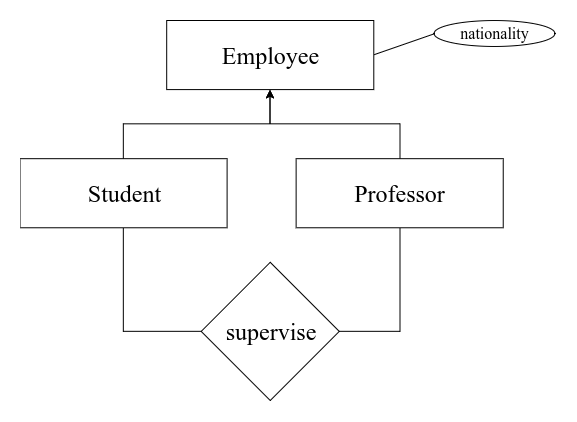
\includegraphics[width=0.8\textwidth]{er1.png}
\end{center}
\caption{Schema E/R}
\end{figure}

Una possibile TBox per lo schema è la seguente:
$\lbrace
Professor \sqsubseteq Employee,
Student \sqsubseteq Employee,
Professor \equiv \forall supervises. Student
\rbrace
$

Il database contiene le seguenti tuple:\\
\textbf{Student:} $(Joe, Italian)$, $(Jill, American)$, $(James, Canadian)$\\
\textbf{Professor:} $(Foo, Mexican)$

Sono verificate le seguenti relazioni:
\textbf{supervise}: $\langle Foo, Joe\rangle, \langle Foo, Jill\rangle$

Una ABox che contiene i dati sopra indicati ed è consistente con la TBox è la seguente: $\big\{ Student(Joe), Student(Jill), Student(James), Professor(Foo),\allowbreak Nationality(Joe, Mexican), Nationality(Jill, American),\allowbreak Nationality(James, Canadian),\allowbreak Nationality(Foo, Mexican),\allowbreak Supervise(Foo, Joe), Supervise(Foo, Jill) \big\}$

\subsection{Queries}

Queries di \textbf{selezione} sul database si possono in generale tradurre come \textit{reasoning task} sulla ABox del tipo \textbf{instance retrieval}.

\textbf{Esempio:} \textit{(si consideri $T, A$ la TBox e la ABox dell'esempio precedente)}\\
NL Query: Who are the mexican employees?\\
DL Query: $T, A \models Employee \sqcap \exists Nationality.Mexican$\footnote{Questa formalizzazione restituirebbe anche employee con più nazionalità, fra cui quella messicana. Alternativamente, $T, A \models Employee \sqcap \forall Nationality.Mexican$ restituirebbe gli employee con nazionalità messicana, \textit{o nessuna nazionalità}.}\\
Answer: $\{Joe, Foo\}$
\\

Le queries che richiedono una risposta affermativa o negativa possono essere tradotte come \textit{instance checking}:
\textbf{Esempio:}
NL Query: Is Joe mexican?\\
DL Query: $T, A \models Nationality(Joe, Mexican)$
Answer: YES (la relazione è contenuta direttamente nella ABox).

\textbf{Esempio:}
NL Query: Is Joe american?\\
DL Query: $T, A \models Nationality(Joe, American)$
Answer: NO se si assume un mondo chiuso (CWA), nulla può dirsi se si assume un mondo aperto (OWA).


\end{document}